\documentclass[10pt,a4paper]{article}
\usepackage[margin=2.3cm]{geometry}
\usepackage[T1]{fontenc}
\usepackage{lmodern}
\usepackage{amsmath,amssymb,amsthm,mathtools}
\usepackage{booktabs,multirow,array,tabularx}
\usepackage{graphicx,xcolor}
\usepackage{tikz}
\usetikzlibrary{arrows.meta,positioning,shapes.geometric,fit,calc,backgrounds}
\usepackage{pgfplots}
\pgfplotsset{compat=1.17}
\usepackage{listings}
\usepackage[numbers,sort&compress]{natbib}
\usepackage[hidelinks]{hyperref}
\usepackage{microtype}
\usepackage{enumitem}
\usepackage{caption}
\usepackage{pifont}

\setlist{itemsep=2pt,topsep=4pt}
\captionsetup{font=small,labelfont=bf}
\renewcommand{\arraystretch}{1.05}

\definecolor{irblue}{RGB}{37,99,235}
\definecolor{llmorange}{RGB}{217,119,6}
\definecolor{detgreen}{RGB}{22,128,60}
\definecolor{lightgrey}{RGB}{243,244,246}

\lstset{basicstyle=\ttfamily\footnotesize,breaklines=true,frame=single,backgroundcolor=\color{lightgrey},
  rulecolor=\color{black!25},columns=fullflexible,keepspaces=true,showstringspaces=false,xleftmargin=2pt,xrightmargin=2pt}

\newcommand{\femagent}{\textsc{femagent}}
\newcommand{\dealii}{\texttt{deal.II}}
\newcommand{\code}[1]{\texttt{#1}}
\newcommand{\cmark}{\ding{51}}
\newcommand{\xmark}{\ding{55}}
\newcommand{\dd}{\,\mathrm{d}}
\DeclareMathOperator{\tr}{tr}
\DeclareMathOperator{\divg}{div}

\title{\femagent: Verification-Driven Translation of Scientific Papers into\\
\dealii{} Finite-Element Solvers through a Typed PDE Intermediate Representation}
\author{\textit{[Author names and affiliations to be inserted]}}
\date{\today}

\begin{document}
\maketitle

\begin{abstract}
Turning the equations of a scientific paper into a trustworthy finite-element code is slow and error-prone. Recent systems let a large language model (LLM) write the solver directly; they are reported to produce code that runs but solves the wrong physics, and production C++ libraries such as \dealii{} are among the hardest targets. We present \femagent{}, a framework in which the language model \emph{never writes solver code}. The model transcribes the paper into a typed, physics-aware PDE intermediate representation (fields, tensor ranks, SI dimensions, boundary and initial conditions, constitutive relations, invariants, provenance), which is strictly separated from the numerical problem data and from discretization choices. A deterministic layer then validates the representation, derives weak forms, time discretizations and Gateaux linearizations, generates complete \dealii{} programs (steady and transient; scalar, vector-valued, nonlinear and coupled; with adaptive meshes, Newton solvers and block preconditioning), and \emph{generates the verification}: manufactured solutions, tangent consistency, declared invariants, structural tests, static well-posedness checks, and mutation testing of the verification itself. We evaluate the paper-to-representation step with locally served open-weight models. From a saved web page of a NAFEMS-derived heat-transfer benchmark, a 27B-parameter model yields a verified solver whose value at the reference point agrees with the published one to $2\cdot10^{-4}$ on converged meshes. In a 60-run benchmark (five LLMs, six documents, HTML and PDF text), 55\% of the extractions passed the deterministic checks and 32\% were equivalent to the ground truth, decided by evaluating the extracted mathematics rather than by string matching; of the 14 extractions that passed the checks but were wrong, 13 were stopped by later layers and one produced a solution of a different problem. Extending the prompt contract to the full vocabulary of the representation raised the number of correct extractions from 8 to 14 of 24, and a toy direct-generation baseline did not produce a compiling \dealii{} program. We discuss the limits of the present prototype---a transparent reference backend on rectangular domains, no matrix-free or MPI backend yet, a small and partly synthetic corpus---and the planned extension to matrix-free HPC operators cross-checked against the reference backend.

\medskip\noindent\textbf{Keywords:} finite element method, \dealii{}, large language models, scientific software engineering, intermediate representation, verification, manufactured solutions, mutation testing.
\end{abstract}

\section{Introduction}
\label{sec:intro}

Most of the quantitative knowledge of computational science is published as papers: a partial differential equation (PDE), a set of boundary and initial conditions, a handful of material parameters, a geometry, and, if the authors are generous, a reference value to compare with. Turning such a description into a working, trustworthy simulation code is a recurring, expensive and error-prone activity. The mathematical content has to be understood, a weak formulation derived, an element and a solver chosen, the boundary treatment implemented, and the result checked against something. Each step is a place where a sign, a factor or a boundary condition can silently go wrong, and a simulation that compiles, runs and converges can still solve a different problem from the one in the paper.

Large language models (LLMs) have changed what can be automated in this chain. They read scientific text well, they write code in many languages, and they can be embedded in loops that compile, run and repair. A series of recent systems apply this to simulation (Section~\ref{sec:review}). Yet the evidence collected so far points to a structural weakness of the dominant architecture, in which the model is asked to produce the simulation code (or the solver input deck) directly: execution success is a poor proxy for scientific correctness \citep{wrongphysics2026,fembench2025}, and the harder and more performance-oriented the target library, the lower the success rate \citep{pdeagentbench2026}.

This paper presents \femagent{}, a research framework that takes a different route. The central design decision is \emph{not} to let a language model write the solver. The model is used for the one task that really needs language understanding, namely reading the paper and filling in a \emph{typed, physics-aware intermediate representation} (the PDE-IR). Everything downstream, i.e.\ the derivation of the weak form, time discretization, linearization, code generation for \dealii{} \citep{arndt2023}, and verification, is deterministic computation on that representation. The representation is also the contract at which the model's output is accepted or rejected: it is checked for referential, rank, dimensional, boundary-completeness and well-posedness consistency, and any inconsistency is returned to the model as a compact structured diagnostic. The principle can be summarised as \emph{the LLM proposes, the deterministic layer disposes}.

\subsection{Existing agentic workflows for scientific software}
\label{sec:review}

\paragraph{General-purpose code agents.}
Code-generation models \citep{codex2021} made program synthesis practical, and agent loops that interleave reasoning with tool use and observation \citep{react2023,reflexion2023} made it iterative. Repository-level benchmarks such as SWE-bench \citep{swebench2024} measure whether an agent can resolve real software issues, where the acceptance criterion is a test-suite that already exists. Closest in spirit to our starting point are systems that turn \emph{papers} into software: Paper2Code/PaperCoder \citep{paper2code2025} transforms machine-learning papers into repositories through planning, analysis and generation agents, and PaperBench \citep{paperbench2025} evaluates the replication of 20 ICML papers against hierarchical rubrics. Their domain is machine learning, where the paper describes an algorithm and the ground truth is a program or a metric; for numerical PDE software the paper describes \emph{mathematics}, and correctness is a property of the discrete solution, which no rubric on source code can establish.

\paragraph{Agents that operate simulation packages.}
A second family lets an LLM \emph{drive} an existing simulation tool. MechAgents \citep{mechagents2023} uses collaborating LLM agents to write, run and self-correct finite-element code for elasticity problems. MetaOpenFOAM \citep{metaopenfoam2024} and Foam-Agent \citep{foamagent2026} generate OpenFOAM cases from natural language, combining retrieval over tutorials and reviewer loops; Foam-Agent additionally exposes its capabilities through the Model Context Protocol (MCP) \citep{mcp2024}. FEABench \citep{feabench2025} evaluates agents that operate the commercial COMSOL Multiphysics package through its API. AutoMOOSE \citep{automoose2026} orchestrates six specialised agents for phase-field simulations in the MOOSE framework \citep{permann2020}, including a ``Skeptic'' that tests results against conservation laws and asymptotic limits. These systems demonstrate that agentic automation of the simulation lifecycle is feasible, and AutoMOOSE in particular shows the value of physics-grounded falsification. Their input is, however, a natural-language request, not the mathematics of a paper, and the artefact the LLM produces is a configuration or input deck for a mature package that already contains the discretization.

\paragraph{LLMs that write finite-element code.}
ALL-FEM \citep{allfem2026} fine-tunes open-weight models (3B--120B parameters) on a corpus of verified FEniCS scripts and embeds them in a multi-agent workflow with runtime feedback; it reports 71.8\% code-level success on 39 benchmarks and shows that fine-tuned, smaller models can compete with a non-agentic frontier model. LLM-PDEveloper \citep{pdeveloper2025} targets \emph{secondary developers}: it translates mathematical and algorithmic descriptions into new solvers or modules of a PDE library and analyses syntactic and semantic failure mechanisms. CodePDE \citep{codepde2025} frames PDE solving as code generation and studies reasoning, debugging, self-refinement and test-time scaling. All three let the model write the numerical code, at the level of scripts or library modules. PDEAgent-Bench \citep{pdeagentbench2026} provides 645 instances for DOLFINx, Firedrake and \dealii{} and evaluates generated solvers in stages: executability, accuracy and efficiency. Its central finding is that models often produce runnable code, but pass rates fall substantially once accuracy and efficiency are required; \dealii{} yields the lowest pass rates of the three libraries: in the single-shot setting the best model reaches $54.1\%$ on the DOLFINx track but only $32.3\%$ on the \dealii{} track, and three attempts with execution feedback raise one strong model on \dealii{} from $19.2\%$ to $26.8\%$. FEM-Bench \citep{fembench2025} evaluates function and unit-test writing for computational mechanics and treats self-verification as a capability of its own.

\paragraph{Verification of generated simulation code.}
The most direct evidence for the problem we address is the \emph{comprehension--generation gap} described by Song et al.\ \citep{wrongphysics2026}: on MooseBench (220 multiphysics cases), 39--40\% of all cases remained runnable but still encoded the wrong physics after execution-only repair, so executability and intent fidelity are separable failure modes. Their remedy reconstructs the PDE encoded by the generated MOOSE objects and compares it with an intended contract (the Intent Fidelity Score). This is a \emph{post hoc} audit of generated code; it presupposes the contract and the code, and works on a structure (Kernels and BCs) that maps compositionally to weak-form terms. Classical computational science has long had the necessary tools for deterministic verification---the method of manufactured solutions (MMS) \citep{roache1998,salari2000,oberkampf2010}, convergence-order tests, and conservation checks---and software engineering has mutation testing as a measure of test-suite quality \citep{demillo1978,jia2011}. What has not been done is to \emph{generate} such verification from a typed mathematical specification extracted from a paper and to use it as the acceptance gate of an LLM-assisted pipeline.

\subsection{Gaps and motivation}
\label{sec:gaps}

Table~\ref{tab:landscape} places these lines of work along the axes that matter for our goal. We read the entries from the cited abstracts and use ``not reported'' where the cited work does not claim the property.

\begin{table}[t]
\centering\small
\caption{Positioning of recent work along the axes relevant to paper-to-solver translation. Entries are taken from the cited publications; ``--'' means the property is not part of the reported approach.}
\label{tab:landscape}
\setlength{\tabcolsep}{3.5pt}
\begin{tabularx}{\textwidth}{@{}p{2.55cm}p{2.25cm}p{2.5cm}p{2.5cm}p{2.7cm}p{1.8cm}@{}}
\toprule
 & Input & LLM output & Target & Verification & Typed math IR\\
\midrule
Paper2Code \citep{paper2code2025} & ML paper & code repository & ML code & model-based and human evaluation & --\\
MetaOpenFOAM, Foam-Agent \citep{metaopenfoam2024,foamagent2026} & NL request & OpenFOAM case files & OpenFOAM & run success, reviewer loop & --\\
AutoMOOSE \citep{automoose2026} & NL request & MOOSE input & MOOSE & physics ``Skeptic'' & --\\
FEABench \citep{feabench2025} & NL problem & API calls & COMSOL & numeric answers & --\\
ALL-FEM \citep{allfem2026} & PDE statement & FEniCS script & FEniCS & runtime feedback & --\\
LLM-PDEveloper \citep{pdeveloper2025} & math/algorithm text & solver/module code & PDE library & success rates, error analysis & --\\
CodePDE \citep{codepde2025} & PDE task & solver code & numerical solvers & reference solution & --\\
PDEAgent-Bench \citep{pdeagentbench2026} & PDE spec & solver code & DOLFINx, Firedrake, \dealii{} & accuracy, runtime targets & --\\
Intent verification \citep{wrongphysics2026} & intended PDE contract & MOOSE input & MOOSE & IFS on encoded PDE & reconstructed\\
\midrule
\textbf{\femagent{} (this work)} & \textbf{scientific paper (web page or PDF text)} & \textbf{typed PDE-IR as JSON; no solver code} & \textbf{\dealii{} C++ (generated)} & \textbf{generated from the IR: MMS, tangent, invariants, mutation} & \textbf{yes}\\
\bottomrule
\end{tabularx}
\end{table}

From the survey we distil five gaps.
\begin{enumerate}[label=\textbf{G\arabic*.},leftmargin=*]
\item \textbf{The input is rarely a paper.} Most pipelines start from a curated prompt or a PDE statement; the extraction of governing equations, boundary conditions and numerical data from the publication, with its notational and structural variety, is left to the user.
\item \textbf{There is no enforceable mathematical contract.} When the model writes code, the only artefact that can be inspected is the code. A typed representation of the mathematics, with rank, dimension and referential rules, turns many extraction errors into immediate, machine-readable diagnostics.
\item \textbf{Mathematical derivations are delegated to the model.} Integration by parts, boundary-term bookkeeping, time discretization and linearization are deterministic transformations. Asking the model to perform them freely invites precisely the sign and factor errors that are so hard to see in code.
\item \textbf{Verification is not derived from the mathematics.} Tests are either given by the benchmark or written by the model, and \emph{passing code} is weak evidence \citep{fembench2025}. Physics-aware checks (convergence order against a manufactured solution, tangent consistency, conservation and dissipation, operator symmetry) can be generated mechanically from the specification, and their power can be quantified by mutation testing.
\item \textbf{Production C++ libraries are neglected.} Python-level libraries dominate the literature, while \dealii{} is reported to be substantially harder for current agents \citep{pdeagentbench2026} (lowest pass rates of the three libraries; see above). A solver for a production C++ library with distributed linear algebra, adaptive meshes and Newton solvers is not a script that an LLM can reliably write monolithically.
\end{enumerate}
A sixth, practical concern cuts across all five: \textbf{auditability and cost.} If every extracted equation, boundary condition and value can be traced to the paper, and if a repair step costs a few hundred tokens of structured diagnostics instead of a whole program and a compiler log, then local open-weight models become realistic for a task that currently invites frontier-model budgets.

\subsection{Contributions}
\label{sec:contrib}
The contributions of this paper are as follows.
\begin{itemize}
\item We present a \textbf{physics-aware PDE intermediate representation} with expression trees, tensor ranks, function spaces, SI dimensions, boundary and initial conditions, constitutive relations, invariants, provenance and ambiguity, strictly separated from the \emph{problem instance} (numbers, geometry) and from discretization choices (Sections~\ref{sec:ir} and \ref{sec:overview}).
\item We describe a \textbf{deterministic mathematical compiler} (strong-to-weak form, time stepping, Gateaux linearization with Newton/Picard) and a \textbf{\dealii{} reference backend} that generates complete C++ programs for steady and transient, scalar, vector-valued, nonlinear and coupled problems, including adaptive mesh and time-step control and block preconditioning (Sections~\ref{sec:compiler} and \ref{sec:backend}).
\item We describe a \textbf{verification framework generated from the IR}: MMS and convergence orders, tangent consistency, declared invariants, structural operator tests, static well-posedness checks and physics mutation testing (Section~\ref{sec:verification}).
\item We define an \textbf{LLM extraction layer} with a provider-agnostic model interface, validation--repair loop and an explicit trust boundary, which works with local open-weight models (Section~\ref{sec:llm}).
\item We report an \textbf{empirical study} of the paper-to-IR step: an end-to-end run on a NAFEMS-derived heat-transfer benchmark with a mesh study against its published reference value, and a 60-run extraction benchmark (five LLMs, six documents, two input formats) scored by \emph{evaluating} the extracted mathematics rather than by string matching, together with an experiment on how much the prompt contract matters (Section~\ref{sec:experiments}).
\end{itemize}
We are explicit about scope. The present implementation targets rectangular two-dimensional domains, polynomial data, continuous Lagrange elements, and a transparent assembled reference backend. The matrix-free/MPI backend, the MCP interface, a curated library of \dealii{} recipes, and the full ablation across architectures are planned but not yet implemented (Section~\ref{sec:outlook}); we do not claim results for them.

The remainder of the paper is organised as follows. Section~\ref{sec:overview} gives the architecture. Sections~\ref{sec:ir}--\ref{sec:verification} describe the representation, the compiler, the backend and the verification. Section~\ref{sec:llm} describes the LLM layer. Section~\ref{sec:experiments} presents the experiments, Section~\ref{sec:discussion} discusses what distinguishes the approach and how to apply it, and Section~\ref{sec:conclusions} concludes with an outlook.

\section{Architecture and Design Principles}
\label{sec:overview}

\paragraph{Design principles.}
The architecture follows five principles that respond directly to the gaps of Section~\ref{sec:gaps}.
\begin{enumerate}[label=\textbf{P\arabic*.},leftmargin=*]
\item \textbf{Do not let the language model write the solver.} A direct ``paper $\to$ LLM $\to$ large \dealii{} program $\to$ compile/fix loop'' architecture is explicitly avoided. The model emits \emph{data} (a JSON document conforming to a schema), never numerical code.
\item \textbf{A typed mathematical IR is the central artefact.} Fields, parameters, strong-form equations, boundary and initial conditions, constitutive laws, energies/invariants, assumptions and provenance live in one validated object. Mathematics, problem data and discretization are kept apart.
\item \textbf{Deterministic where mathematics is deterministic.} Integration by parts, time discretization, linearization, code generation and verification are ordinary programs whose behaviour is reproducible and unit-testable. The LLM never skips the IR to go to the weak form or to code.
\item \textbf{Verification is derived from the specification.} Tests are generated from the IR (manufactured solutions, tangent checks, invariants, structural checks), and their quality is itself measured (mutation testing).
\item \textbf{The model is a replaceable component behind a narrow interface.} A single abstract method (\code{complete}) separates the framework from any provider; remote, local OpenAI-compatible and scripted test doubles are interchangeable.
\end{enumerate}

\paragraph{Pipeline.}
Figure~\ref{fig:arch} shows the end-to-end flow. A paper (a saved publisher web page with MathML equations, or text extracted from a PDF) is flattened into prompt text. The language model is asked twice: first for the \code{PDEModel} (the mathematics), then, given the declared parameters and boundary names, for the \code{ProblemInstance} (numerical values and the domain). Both answers pass through the deterministic \emph{trust boundary}. Schema parsing, referential, rank and dimension validation (model) and instance completeness checks (instance) are inside the repair loop: failures are returned to the model as short structured diagnostics for up to three attempts. The static well-posedness and plan checks (inf--sup pairing, pinning, boundary-flux sign, time plan) run at the \code{validate} stage of the pipeline, after extraction, and report to the user, who can edit the stored JSON. Accepted objects feed the deterministic chain: weak form, time/linearization, \dealii{} code generation, build, run, diagnostics and the verification gate. Every intermediate result is stored (\code{model.json}, \code{instance.json}, raw LLM answers, generated \code{main.cc}, solution, report), so a wrong extraction can be corrected by hand and the run resumed from the edited JSON \emph{without} calling the model again.

\begin{figure}[t]
\centering
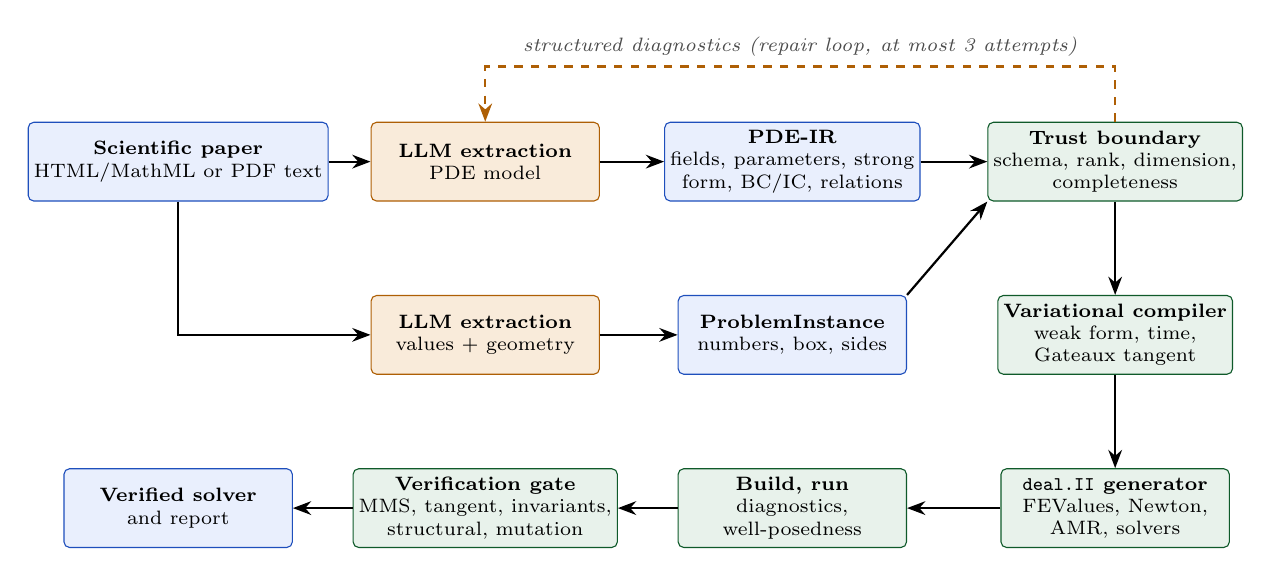
\begin{tikzpicture}[
  box/.style={draw,rounded corners=2pt,align=center,minimum height=10mm,minimum width=29mm,inner sep=2pt,font=\scriptsize},
  llm/.style={box,fill=llmorange!15,draw=llmorange!80!black},
  det/.style={box,fill=detgreen!10,draw=detgreen!70!black},
  art/.style={box,fill=irblue!10,draw=irblue!80!black},
  arr/.style={->,>=Stealth,thick},
  lab/.style={font=\scriptsize\itshape,text=black!70}]
\node[art] (paper) at (0,0) {\textbf{Scientific paper}\\ HTML/MathML or PDF text};
\node[llm] (ex1) at (3.9,0) {\textbf{LLM extraction}\\ PDE model};
\node[art] (ir) at (7.8,0) {\textbf{PDE-IR}\\ fields, parameters, strong\\ form, BC/IC, relations};
\node[det] (val) at (11.9,0) {\textbf{Trust boundary}\\ schema, rank, dimension,\\ completeness};
\node[llm] (ex2) at (3.9,-2.2) {\textbf{LLM extraction}\\ values + geometry};
\node[art] (inst) at (7.8,-2.2) {\textbf{ProblemInstance}\\ numbers, box, sides};
\node[det] (weak) at (11.9,-2.2) {\textbf{Variational compiler}\\ weak form, time,\\ Gateaux tangent};
\node[det] (gen) at (11.9,-4.4) {\textbf{\dealii{} generator}\\ FEValues, Newton,\\ AMR, solvers};
\node[det] (build) at (7.8,-4.4) {\textbf{Build, run}\\ diagnostics,\\ well-posedness};
\node[det] (ver) at (3.9,-4.4) {\textbf{Verification gate}\\ MMS, tangent, invariants,\\ structural, mutation};
\node[art] (out) at (0,-4.4) {\textbf{Verified solver}\\ and report};
\draw[arr] (paper)--(ex1);
\draw[arr] (ex1)--(ir);
\draw[arr] (ir)--(val);
\draw[arr] (paper.south)--++(0,-0.0)|-(ex2.west);
\draw[arr] (ex2)--(inst);
\draw[arr] (inst.north east)--(val.south west);
\draw[arr] (val)--(weak);
\draw[arr] (weak)--(gen);
\draw[arr] (gen)--(build);
\draw[arr] (build)--(ver);
\draw[arr] (ver)--(out);
\draw[arr,dashed,llmorange!80!black] (val.north)--++(0,0.7)-|(ex1.north) node[lab,pos=0.25,above] {structured diagnostics (repair loop, at most 3 attempts)};
\end{tikzpicture}
\caption{Architecture of \femagent{}. Orange boxes are the only steps that call a language model; green boxes are deterministic; blue boxes are typed artefacts that are stored, inspected and editable. The language model never produces solver code.}
\label{fig:arch}
\end{figure}

\paragraph{Separation of concerns.}
Three kinds of information are kept in three different objects (ADR~0002 in the repository). The \code{PDEModel} holds mathematics only and no numbers. The \code{ProblemInstance} holds the numerical values of the parameters, the domain (an axis-aligned box and a map from each IR boundary name to mesh sides) and a short free-text source note per value. The \emph{discretization plan} holds everything that a paper does not state: element degrees, time-stepping scheme and step, linear solver and preconditioner, Newton globalization, adaptivity. This separation has three consequences: the mathematics can be verified without choosing a mesh; the discretization can be changed without touching the extraction; and the system can state \emph{exactly} what is missing (a parameter value, a boundary mapping) before any code is generated, instead of failing late inside code generation.

\paragraph{Why the architecture suits small models.}
The model's task is reduced to \emph{transcription into a schema}, with a checker in the loop. The prompt for the PDE model has about 3\,000 tokens including the schema example (Section~\ref{sec:experiments}), and a repair message is a list of one-line diagnostics. We hypothesise, and test in Section~\ref{sec:experiments}, that this makes the task feasible for locally served 8--30B-parameter models, while the same models would be unlikely to write several hundred lines of correct \dealii{} C++.

\section{The Physics-Aware PDE Intermediate Representation}
\label{sec:ir}

\subsection{Expressions and models}
The PDE-IR is a typed, serialisable tree language plus an outer record. Expression nodes are immutable dataclasses; every node can carry optional \code{provenance} and \code{ambiguity} annotations that do not take part in structural equality. Table~\ref{tab:nodes} lists the node families. The vocabulary is deliberately small: it covers the operators of the continuum-mechanics and phase-field problems targeted in the first release, and each node has a defined tensor rank, a printer (text and \LaTeX), a JSON codec, a weak-form rule and, where applicable, a differentiation rule.

\begin{table}[t]
\centering\small
\caption{Expression nodes of the PDE-IR.}
\label{tab:nodes}
\begin{tabularx}{\textwidth}{@{}p{3.1cm}X@{}}
\toprule
Family & Nodes\\
\midrule
Leaves & \code{Constant}, \code{Field} (name, rank, function space, SI dimension), \code{Parameter} (name, rank, dimension), \code{SpatialCoordinate}(axis), \code{TimeCoordinate}, \code{Normal}, \code{Identity}\\
Algebra & \code{Add}, \code{Mul}, \code{Neg}, \code{Pow}, \code{VectorExpr}, \code{Inner}, \code{Transpose}, \code{Trace}\\
Differential operators & \code{Grad}, \code{Div}, \code{Laplacian}, \code{TimeDerivative}, \code{Convection} ($(\mathbf a\cdot\nabla)\,b$)\\
Constitutive & \code{Apply}(name, arguments, rank), resolved through named relations $\mathrm{name}(\text{formals})=\text{body}$ with simultaneous substitution\\
Variational & \code{DomainIntegral}, \code{BoundaryIntegral}, \code{Equation} (lhs, rhs)\\
\bottomrule
\end{tabularx}
\end{table}

A \code{PDEModel} bundles \code{fields}, \code{parameters}, \code{equations}, \code{initial\_conditions}, \code{boundary\_conditions} (Dirichlet, Neumann, Robin; each with a field, a boundary name and an expression value), \code{constitutive\_relations}, \code{invariants} (an expression, a behaviour---conserved, non-increasing, non-decreasing, positive---and a tolerance), free-text \code{assumptions}, and model-level provenance and ambiguity. The IR deliberately encodes the \emph{strong} form: the weak form is derived by the compiler.

\paragraph{Boundary-condition convention.}
A Dirichlet value is the prescribed field value. A Neumann or Robin value is the prescribed \emph{outward normal flux} of the diffusive flux appearing in the equation, so that for $-\nabla\cdot(k\nabla T)=0$ the value is $k\,\partial_n T$. Consequently an insulated boundary is a Neumann condition with value $0$, and Newton's law of cooling $-k\,\partial_n T=h\,(T-T_\infty)$ is a Robin condition with value $-h\,(T-T_\infty)$. This convention is stated in the extraction prompt; Section~\ref{sec:experiments} shows that mistakes against it are the kind of error that actually occurs.

\paragraph{Example.}
The heat-transfer benchmark of Section~\ref{sec:heat} is represented by the model below, as printed by the IR's text printer (the JSON form is about 150 lines because every \code{Field} and \code{Parameter} leaf carries its metadata):
\begin{lstlisting}
fields:       T            (scalar, H1, [temperature])
parameters:   k  [W/(m K)],  h  [W/(m^2 K)],  T_amb  [K]
equation:     div(grad(T) * k) = 0
BC bottom         dirichlet  100
BC left           neumann    0
BC top_and_right  robin      -(h * (T - T_amb))
\end{lstlisting}

\subsection{Function spaces, ranks and dimensions}
Every \code{Field} declares a function space (H1, H(div), H(curl), L2) and a tensor rank (scalar, vector, tensor). The space is part of the mathematical specification (which regularity does the unknown have?), while the polynomial degree and element family are \emph{discretization} data kept in the plan or the instance. Dimensions are vectors of integer exponents of the seven SI base quantities, with an algebra for products, quotients and powers. Rank inference is shared with the weak-form compiler so that the validator and the compiler agree.

\subsection{Provenance and ambiguity}
Each node, boundary condition, initial condition, constitutive relation, invariant and model can be annotated with a \code{Provenance} (document, equation label, page, the transformation applied, and a note) and with an \code{Ambiguity} (confidence, reason, textual alternative readings with their own confidence, and a resolved flag). Transformations extend provenance rather than replace it: the weak form derived from the equation labelled (1) carries \code{transformation = integration\_by\_parts} and a note recording why a boundary term vanished (for instance, ``test function vanishes on the Dirichlet part''). This is the basis for answering where a term came from and why a boundary integral was eliminated. At the instance level, \code{value\_sources} records one short note per parameter value (``Governing equation section: $k=52$''). We note honestly that provenance is fully \emph{supported} by the data model but, in the current LLM layer, populated only through these value notes; asking the model to attach page/equation provenance to every node is part of the outlook.

\subsection{The trust boundary: validation}
\label{sec:validation}
The validators return structured \code{ValidationIssue} records (code, severity, message, location) rather than raising, so that the same diagnostics serve humans and the repair loop. Table~\ref{tab:validators} lists the categories.

\begin{table}[t]
\centering\small
\caption{Deterministic checks at the trust boundary (issue codes in the implementation).}
\label{tab:validators}
\begin{tabularx}{\textwidth}{@{}p{2.9cm}p{3.6cm}X@{}}
\toprule
Level & Codes & Meaning\\
\midrule
Schema & parse errors, \code{missing key} & JSON is not a valid \code{PDEModel}; the message names the offending key or the non-integer dimension exponents\\
Referential & undeclared field/parameter & every symbol used in an equation, relation, invariant or BC is declared\\
Rank & \code{rank\_mismatch}, \code{div\_of\_scalar}, \code{trace\_of\_non\_tensor}, \code{convection\_velocity\_not\_vector} & terms of a sum and the two sides of an equation have one tensor rank; operators are applied to admissible ranks\\
Dimension & \code{dimension\_mismatch} & terms of a sum and equation sides have equal SI dimension; deliberately conservative: only two \emph{known, differing} dimensions are flagged\\
Time & \code{missing\_time\_plan}, \code{missing\_num\_steps}, time coordinate without a time derivative, missing initial data & the time structure of the model matches the plan\\
Instance & \code{missing\_parameter\_value}, \code{parameter\_value\_shape}, \code{missing\_boundary\_mapping}, \code{unconstrained\_sides}, \code{overlapping\_boundaries} & every declared parameter has a value of the right shape; every named boundary is mapped to mesh sides without overlap\\
Well-posedness & \code{inf\_sup\_violation}, \code{multiplier\_not\_pinned}, \code{anti\_dissipative\_boundary} & see below\\
\bottomrule
\end{tabularx}
\end{table}

The \emph{well-posedness} checks read the model against the discretization plan, statically, without building anything. (i)~For a constraint multiplier such as the pressure of an incompressible flow, the multiplier space must be smaller than the space it constrains (the inf--sup condition \citep{boffi2013}); equal-order pairs such as $Q_2/Q_2$ are rejected, and Taylor--Hood degrees \citep{taylorhood1973} are suggested. (ii)~A multiplier that sees only Dirichlet data on the field it constrains is determined up to a constant, so the instance must pin it; conversely, pinning with an open boundary over-constrains it. (iii)~A Neumann or Robin value $q\cdot n$ of a diffusive flux must not \emph{grow} with the unknown: $-k\,\partial_n u = h(u-u_\infty)$ must be encoded as $-h(u-u_\infty)$; the opposite sign feeds energy through the boundary and is almost always a sign error in the extraction. This last rule is the direct result of an observed failure: when the pipeline was first tried on the heat benchmark with a local model, the model emitted $h\,T - T_\infty$ with the wrong sign, which the generator would have compiled and solved without complaint; the check now reports \code{anti\_dissipative\_boundary} and quotes the correct form in its message. (The message is written for the person who edits \code{model.json}; these static checks currently run at the \code{validate} stage and are not yet part of the model's repair loop, which uses the schema, rank, dimension and instance-completeness checks.)

\subsection{Problem instance}
The instance carries \code{parameter\_values} (a float, or a list of floats for vector parameters), a \code{RectangleGeometry} (lower-left and upper-right corner, a map from boundary names to \dealii{} colorize ids---$0$/$1$ for $x_{\min}/x_{\max}$, $2$/$3$ for $y_{\min}/y_{\max}$---and the number of global refinements), \code{field\_degrees} and \code{pin\_fields} (the small amount of spatial discretization data that a mixed problem needs), and \code{value\_sources}. \code{check\_problem\_instance} reports missing values and unmapped boundaries as errors and a missing geometry as a warning (a placeholder mesh is used). One boundary name may cover several sides (for example \code{top\_and\_right}$\mapsto[1,3]$), in which case the generator relabels the sides to one mesh id.

\section{The Deterministic Mathematical Compiler}
\label{sec:compiler}

\subsection{From the strong form to the weak form}
The compiler turns each strong-form equation $\mathcal L(u)=0$ into a residual $R(u;v)=0$ for test functions $v$ in the space of the corresponding unknown. It applies the following rules, each tagged in the provenance of the result.
\begin{enumerate}
\item \emph{Test and integrate.} Multiply by a test function of matching rank (scalar $v$ for scalar equations, vector $\mathbf v$ for vector equations; a vector equation uses the inner product) and integrate over $\Omega$.
\item \emph{Integrate by parts} every divergence term of second order, $-\int_\Omega\nabla\cdot\mathbf q\,v\dd x=\int_\Omega\mathbf q\cdot\nabla v\dd x-\int_{\partial\Omega}(\mathbf q\cdot\mathbf n)\,v\dd s$, where $\mathbf q$ is a vector flux ($\mathbf q=k\nabla u$) or, for a tensor flux, $\sigma(u):\nabla\mathbf v$ and $(\sigma\mathbf n)\cdot\mathbf v$. A \code{Laplacian} is first rewritten as a divergence of a gradient. Terms of first order (for instance a pressure gradient $\nabla p\cdot\mathbf v$ or a convection term) are tested but not integrated by parts.
\item \emph{Treat the boundary term} according to the boundary conditions. On a Dirichlet boundary the test function vanishes and the term is dropped (the value is imposed through constraints); on a Neumann boundary $\mathbf q\cdot\mathbf n$ is replaced by the prescribed outward flux $g_N$; on a Robin boundary it is replaced by the value expression, which still references the unknown and therefore contributes a boundary mass term to the matrix and a source-like term to the right-hand side. Boundaries without a stated condition are natural (homogeneous Neumann).
\end{enumerate}
For $-\nabla\cdot(k\nabla u)=f$ with Dirichlet data on $\Gamma_D$ and flux $g_N$ on $\Gamma_N$ the result is
\begin{equation}
\int_\Omega k\nabla u\cdot\nabla v\dd x-\int_\Omega f\,v\dd x-\int_{\Gamma_N}g_N\,v\dd s=0 .
\end{equation}
For the heat benchmark of Section~\ref{sec:heat} with Newton's law of cooling on $\Gamma_R$ ($\mathbf q\cdot\mathbf n=-h(T-T_\infty)$) the result is
\begin{equation}
\int_\Omega k\nabla T\cdot\nabla v\dd x+\int_{\Gamma_R}h\,T\,v\dd s=\int_{\Gamma_R}h\,T_\infty\,v\dd s .
\end{equation}
The compiler does not accept an LLM-supplied weak form; the strong form is the only input. Because the transformation is deterministic, an extraction that writes $\nabla\cdot(k\nabla T)=0$ instead of $-\nabla\cdot(k\nabla T)=0$ yields the same discrete problem, since the flux relation is applied consistently to the equation as written.

\subsection{Time discretization}
A \code{TimeDerivative} makes the model time-dependent, and the discretization plan then selects a time family. The reference backend supports (i)~self-discretized schemes (backward Euler/BDF1, a $\theta$-method, and an IMEX splitting that treats the linear part implicitly and nonlinear reaction terms explicitly), (ii)~\dealii{} Runge--Kutta schemes, and (iii)~a SUNDIALS ARKode family in which the integrator owns the loop. For nonlinear and multi-field problems the system path uses implicit Euler with a Newton solve per step. The residual of the step is built by replacing every $u_t$ by $(u-u^{n})/\Delta t$, which remains valid when $u_t$ has a nonlinear coefficient. Time-varying Dirichlet data (\code{TimeCoordinate} in a boundary value) is re-applied at every step; time-independent data is applied once, so that steady-state code is byte-identical to before. Static checks confirm that a \code{TimeDerivative} comes with a time plan and a step count and that a steady model does not receive one; first-order derivatives of bare fields are required; fields without a time derivative are identified as algebraic (the pressure of an incompressible flow gives an index-two differential--algebraic system), which excludes explicit schemes for them.

\subsection{Gateaux linearization and Newton/Picard}
For nonlinear residuals $R(u;v)=0$ the compiler derives the Jacobian symbolically as the Gateaux derivative
\begin{equation}
J(u)[\delta u;v]=\left.\frac{\mathrm d}{\mathrm d\varepsilon}R(u+\varepsilon\,\delta u;v)\right|_{\varepsilon=0}.
\end{equation}
The linearization engine differentiates \code{Grad}, \code{Div}, \code{Transpose}, \code{Trace}, \code{Inner}, products, powers and constitutive \code{Apply} nodes (relations are inlined; multi-argument relations $k(u,\nabla u)$ are substituted simultaneously and differentiated with the chain rule). Convection is handled as a first-class node: $D[(\mathbf a\cdot\nabla)\mathbf b]=(D\mathbf a\cdot\nabla)\mathbf b+(\mathbf a\cdot\nabla)D\mathbf b$ gives the Newton tangent, and holding the convecting velocity fixed gives a Picard iteration. Choosing a dedicated node rather than a composition of \code{Inner} and \code{Grad} avoids an index ambiguity ($\nabla b\cdot\mathbf a$ against $\mathbf a\cdot\nabla b$ differ for vector $b$). This engine is not left unverified: Section~\ref{sec:verification} describes the tangent-consistency gate that checks, on the very integrands the generated solver uses, that $J(u)\,p\approx(R(u+\epsilon p)-R(u))/\epsilon$ for a perturbation $p$ in each field and in all fields.

\subsection{The discretization plan}
Choices that a paper does not state are collected in a \code{DiscretizationPlan}: time family and scheme; \code{LinearSolverSpec} (direct, CG, GMRES; preconditioner none, SSOR, block-triangular with SIMPLE or scaled LSC Schur complement); \code{NewtonSpec} (full step or residual-based backtracking line search, absolute/relative/step tolerances, iteration limits, divergence and stagnation detection); \code{AdaptiveRefinementSpec} (number of Kelly-estimator cycles, marking strategy, transfer frequency); and \code{TimeStepControlSpec} (relative tolerance for an embedded-pair controller). Static checks reject or warn about specifications that are inconsistent with the model: CG on a nonsymmetric or indefinite operator (\code{cg\_nonsymmetric}, \code{cg\_indefinite}), a block preconditioner on a problem without saddle-point structure, a preconditioner on a zero diagonal, an unpreconditioned iterative solve of a saddle-point system (\code{saddle\_point\_unpreconditioned}), and time-step control requested for a steady model (\code{time\_control\_steady}). Default plans are chosen by \code{plan\_discretization}; elements default to $Q_1$, and to Taylor--Hood $Q_2/Q_1$ for problems with a constraint multiplier.

\section{The \dealii{} Reference Backend}
\label{sec:backend}

\subsection{Scope and structure}
The backend turns a validated \code{(PDEModel, ProblemInstance, DiscretizationPlan)} triple into a complete, self-contained \dealii{} project (a \code{main.cc} and a \code{CMakeLists.txt}). It is the \emph{reference} backend of the research plan: it favours mathematical transparency and ease of debugging over speed, and uses assembled sparse matrices with \code{FEValues}, \code{DoFHandler}, \code{AffineConstraints} and explicit assembly loops. Two generators share the compiler: a scalar path (\code{FE\_Q}, sparse matrix) and a system path (\code{FESystem} with one block per field, used for vector-valued, mixed and coupled models and for every nonlinear model that needs Newton). A third generator emits the Newton-specific code for scalar quasilinear diffusion. Table~\ref{tab:coverage} summarises the classes of problems covered, with the benchmark in the repository that exercises each.

\begin{table}[t]
\centering\small
\caption{Problem classes handled by the reference backend and the repository benchmarks that exercise them. All run end to end on a real \dealii{} installation.}
\label{tab:coverage}
\begin{tabularx}{\textwidth}{@{}p{4.1cm}X@{}}
\toprule
Class & Benchmarks (gold PDE-IR models)\\
\midrule
Linear steady scalar & \code{poisson}, \code{heat\_conduction\_robin} (Dirichlet, Neumann and Robin data)\\
Nonlinear steady scalar & \code{nonlinear\_diffusion} ($-\nabla\cdot(\kappa(u)\nabla u)=f$, Newton)\\
Linear elasticity (vector) & \code{elasticity}, \code{loaded\_beam} (spatially varying traction)\\
Nonlinear elasticity & \code{nonlinear\_elasticity} (Newton on the \code{FESystem}, quadratic convergence)\\
Stokes (mixed) & \code{stokes}, \code{lid\_driven\_cavity}, \code{channel\_flow}\\
Navier--Stokes & \code{navier\_stokes} (Newton and Picard), \code{unsteady\_navier\_stokes}, \code{ramped\_lid\_cavity}\\
Transient linear & \code{transient\_heat} (time-varying Dirichlet data), \code{unsteady\_stokes}\\
Nonlinear coupled transient & \code{nonlinear\_parabolic}, \code{allen\_cahn}, \code{cahn\_hilliard} (two-field $c/\mu$ formulation, Newton per step)\\
\bottomrule
\end{tabularx}
\end{table}

\subsection{Generated solver features}
\paragraph{Boundary data.} Constant and spatially varying scalar and vector data, time-varying Dirichlet and source data, Neumann tractions as vector expressions, and Robin terms are rendered into component-wise quadrature-point expressions. Boundary names that cover several mesh sides are relabelled to one mesh boundary id. Hanging-node constraints are combined with Dirichlet constraints; for time-varying Dirichlet data the Dirichlet part of the constraints is rebuilt every step while the hanging-node part is kept.

\paragraph{Linear solvers.} Direct (UMFPACK \citep{davis2004}), CG with SSOR, and GMRES. For saddle-point systems the backend generates a block upper-triangular preconditioner with an algebraic Schur-complement approximation by SIMPLE \citep{patankar1972} or by the scaled least-squares commutator (LSC) approach \citep{elman2006}. On a lid-driven cavity the LSC variant needed 17, 25 and 38 GMRES iterations on three successively refined meshes: it is not mesh independent and, in two dimensions, not faster than the direct solver, so it is a scalability option rather than a default.

\paragraph{Nonlinear solvers.} Newton with the symbolically derived tangent, with optional residual-based backtracking and robust convergence criteria (absolute and relative residual, step norm, iteration limit, divergence and stagnation detection reported by name). A Reynolds-number-1000 cavity that plain Newton cannot solve converged in 13 iterations with backtracking.

\paragraph{Adaptivity.} Steady problems can be solved on adaptively refined meshes using the Kelly error estimator \citep{kelly1983} with fixed-fraction marking; for a steep manufactured solution the adaptive loop reached the accuracy of uniform refinement with $3.9$--$8.7\times$ fewer degrees of freedom, and for Navier--Stokes it refined at the lid corners. For transient problems an \code{adapt\_mesh()} step with \code{SolutionTransfer} is inserted in the time loop (with initial refinement towards the initial data); for a persistent steep feature the adaptive run had a $3.3\times$ lower error with 37\% fewer cells, but for a quickly decaying bump it did not help. An embedded error estimate (a pair of different order) and a PI controller throttled by the Newton iteration count control the time step.

\paragraph{Diagnostics.} The generated programs print machine-parsable lines (mesh size, Newton residual history and step lengths, linear-solver iteration counts, time-step acceptance and rejection, invariants per step). The pipeline parses them into structured reports and an acceptance gate (\code{diagnose}) that fails, with a named reason, on Newton divergence, stagnation or line-search failure.

\subsection{Pipeline stages and reports}
The orchestrator runs six stages and records each as \code{passed}, \code{failed} or \code{skipped}:
\begin{enumerate}[nosep]
\item \textbf{validate}: IR, instance, time plan, solver plan and well-posedness checks (Section~\ref{sec:validation}).
\item \textbf{generate}: derive the weak form and emit the program; unsupported constructs raise a descriptive error (``unsupported construct: \ldots'') rather than producing partial code.
\item \textbf{build}: configure with CMake against the given \dealii{} installation and compile; the first compiler error is quoted.
\item \textbf{run}: execute; mesh size and solver notes are extracted from the output.
\item \textbf{diagnose}: Newton/linear-solver/time-step acceptance.
\item \textbf{verify}: the verification gate of Section~\ref{sec:verification}, with the applicable checks chosen from the structure of the model.
\end{enumerate}
Stages that need a \dealii{} installation are skipped, not failed, when none is provided, so \code{validate} and \code{generate} run anywhere. For example, the heat benchmark program of Section~\ref{sec:heat} is generated on a mesh of $16\times16$ cells and is a 236-line \dealii{} program, all of it produced from the eight-line IR summary of Section~\ref{sec:ir} and the instance.

\subsection{Limitations of the current backend}
The geometry is an axis-aligned box generated with \code{GridGenerator::hyper\_rectangle} and colorized sides; no unstructured meshes are read yet. The expression language has no transcendental functions, so data are polynomials in the coordinates and time (a separate analytic AST with $\sin$, $\cos$ and $\exp$ is used only inside the verification code to derive forcing terms). Only \code{H1} fields (continuous Lagrange) are generated, and the scalar path currently uses $Q_1$ elements regardless of the requested degree (we observed identical meshes and results for $Q_1$ and $Q_2$ requests on the heat benchmark); higher degrees are available in the system path through \code{field\_degrees}. $\mathrm{H(div)}$, $\mathrm{H(curl)}$ and discontinuous spaces are representable in the IR but rejected by the generator. Time-dependent nonlinear systems use backward Euler. There is no MPI, matrix-free or SIMD backend yet; this is the principal item of future work (Section~\ref{sec:outlook}).

\section{Verification Generated from the Specification}
\label{sec:verification}

The research question behind the framework is not whether a model can emit FEM code, but whether the mathematical specification in a paper can be turned into a \emph{semantically verified} implementation. Compilation and a converged solve are necessary conditions only. The verification package therefore contains tests that are derived from the IR and from the compiled operators, and each of them has been run against the real \dealii{} installation during development. The numbers quoted in this section are those obtained by the development test campaign (documented in the repository) and were not re-measured for this paper, with the exception of the experiments in Section~\ref{sec:experiments}.

\subsection{Manufactured solutions and convergence orders}
The method of manufactured solutions \citep{roache1998,salari2000} chooses a smooth exact solution $u^\star$, derives the forcing that makes it an exact solution of the discrete problem's PDE, imposes the corresponding Dirichlet data, and measures $\|u_h-u^\star\|$ on a sequence of refined meshes. The test checks the \emph{observed order}, not merely that the error decreases: for $Q_p$ elements one expects $p+1$ in $L^2$ and $p$ in $H^1$. In \femagent{} the forcing is derived symbolically by evaluating the IR operators (\code{TimeDerivative}, \code{Grad}, \code{Div}, \code{Laplacian}, \code{Inner}, \code{Convection}, constitutive \code{Apply}) on expanded sparse polynomials in $(x,y,t)$ and converting the result back into IR data. Evaluating on expanded polynomials rather than on factored expressions was necessary: factored symbolic differentiation produced a 2.3~MB generated source file that crashed the compiler. Because the manufactured forcing is injected as ordinary IR data, it is the \emph{generated solver itself} that is verified, not a dedicated driver. Reported results: for the scalar diffusion operator with $u^\star=\sin(\pi x)\sin(\pi y)$ and $Q_1$ elements the observed orders were $2.00$ ($L^2$) and $1.00$ ($H^1$); for the nonlinear parabolic two-field system, implicit Euler had observed temporal orders $0.99$ and $1.00$ and $Q_2$ nodal errors converged with order about $4.1$ and $4.0$ (superconvergence at the nodes); Navier--Stokes was exact for a manufactured polynomial solution with both Newton and Picard iterations.

\subsection{Tangent consistency}
For nonlinear problems a wrong Jacobian typically still converges (slowly) or fails in ways that look like a solver problem. The tangent gate checks
\begin{equation}
J(u)\,p\approx\frac{R(u+\epsilon p)-R(u)}{\epsilon}
\end{equation}
for a sequence of $\epsilon$, using the \emph{same cell integrands} the Newton solver assembles, for a perturbation $p$ in each field separately and in all fields together. A correct tangent shows first-order decay of the discrepancy down to a floor ($1.5\cdot10^{-7}$ for the nonlinear-elasticity benchmark; $2\cdot10^{-14}$, $3\cdot10^{-7}$ and $10^{-7}$ for the velocity, the pressure and all fields of Stokes flow with a pressure-dependent viscosity). A deliberately mutated tangent that drops the pressure coupling of the viscosity stagnates at a discrepancy of $1.0$ for the pressure perturbation and $0.34$ for the combined one, while the velocity block still passes, i.e., the check \emph{localises} the defective block. A tangent that fails does not proceed to later stages.

\subsection{Declared invariants and energies}
Each \code{Invariant} in the IR (an expression, a behaviour and a tolerance) is turned into an integral that the generated transient program evaluates and prints at every step. The checker verifies that a conserved quantity does not drift beyond the tolerance and that a non-increasing quantity (a free energy) never increases between steps. For the Cahn--Hilliard benchmark (two-field $c/\mu$ formulation, $Q_2/Q_2$, 50 backward-Euler steps of size $10^{-3}$, Newton with 3 iterations per step) the mass stays at $5.000000000000\cdot10^{-2}$ and the free energy decreases from $0.248335$ to $0.246706$; for Allen--Cahn (100 steps of size $10^{-2}$, saddle-shaped initial field) the free energy decreases from $0.240069$ to $0.215374$ and mass is, correctly, not conserved. Implicit-Euler energy decay is not unconditional; it holds for these step sizes, and convex splitting would give an unconditional result.

\subsection{Structural tests}
The scalar diffusion operator is checked for symmetry of the assembled stiffness matrix, for the constant null space $K\mathbf 1=0$, and for positive semi-definiteness via the minimal eigenvalue (LAPACK). The measured values were: asymmetry $0$, $\|K\mathbf 1\|\approx3.5\cdot10^{-16}$ and minimal eigenvalue $\approx0$. Further mathematically justified structural properties (rigid-body modes, incompressibility, MPI-rank independence) are planned.

\subsection{Static well-posedness checks}
The checks of Section~\ref{sec:validation} (inf--sup pairing, multiplier pinning, boundary-flux sign, algebraic fields) are verification in the same spirit but require no build; they run at the \code{validate} stage and cost milliseconds.

\subsection{Mutation testing: how good is the verification?}
A test-suite that passes the correct code is weak evidence \citep{demillo1978,jia2011}. \femagent{} therefore injects physically meaningful faults into the \emph{generated operator} and re-runs the verification on each mutant, reporting the mutation score $=$ killed/total, where a mutant is killed by a compile error, a runtime failure or a failing check. The implemented operators are sign flip, dropped operator, wrong (doubled) coefficient, and replacement of diffusion by a reaction term ($\nabla u\to u$); coupled-system mutants (for example dropping a coupling block) exercise the coupled MMS driver. In the real campaign on the diffusion operator all four mutants were killed (score $100\%$). This is a small mutant set and we do not claim a general detection rate; extending the operator catalogue (wrong normal sign, wrong component, replaced trial/test fields) and the benchmark set is part of the outlook. We also report an honest negative result from development: a mutated Cahn--Hilliard mobility with the wrong sign was caught \emph{earlier} than by the invariant gate, because the Newton iteration diverged and the \code{run} stage failed; a mutant caught by the invariant gate itself has not yet been demonstrated.

\subsection{What the gate does not cover}
The verification gate checks the interior operator and, where applicable, the Newton integrand and the invariants. In the current implementation the MMS driver imposes pure Dirichlet data on the unit square, so \emph{boundary-condition treatment} (Robin and Neumann terms) is not exercised by it; the end-to-end experiment of Section~\ref{sec:heat} therefore additionally compares with an independent published reference value. Verification of the extracted \emph{inputs} (that the paper was read correctly) is the task of the validators and of human review of the stored JSON; Section~\ref{sec:extraction} quantifies how often this layer succeeds.

\section{The LLM Extraction Layer}
\label{sec:llm}

\subsection{Model interface}
All model access goes through one abstract class with a single abstract method, \code{complete(messages, temperature, max\_tokens)}. Structured generation, schema parsing and the repair loop are shared and independent of the transport. The concrete transport is an OpenAI-compatible chat endpoint, which covers hosted models and locally served open-weight models (Ollama, vLLM, llama.cpp) through a \code{base\_url}; an offline scripted double supports deterministic tests. Models that expose their reasoning in a separate field (the Qwen3 family and similar) have it captured and stored next to the answer. No model-specific code is present elsewhere in the framework.

\subsection{Paper ingestion}
The preferred input is a saved publisher web page, because publishers embed equations as MathML islands, which are structured and machine-readable, in contrast to the ungrouped glyphs of a PDF or rasterised equation images. The HTML adapter splits the page on headings into sections, keeps paragraph text and every \code{<math>} element as an equation record with a guessed label, and renders the document as plain text with the MathML markup inline. Any other file (for instance text extracted from a PDF, or LaTeX) is read as plain text. The earlier hand-written MathML/LaTeX parsers (``Stage A/B'') were demoted to an optional independent cross-check after they proved fragile and effectively overfitted to a single page (ADR~0001).

\subsection{Extraction prompts}
Two prompts are used, mirroring the two objects.
\begin{description}
\item[Model prompt.] The system prompt states the task (transcribe the model into the PDE-IR), lists the node tags, and states the rules: declare every field and parameter; give the \emph{strong} form; the flux sign convention for Neumann and Robin conditions, with the convective example $-k\,\partial_nu=h(u-u_\infty)\mapsto-h(u-u_\infty)$; one boundary name per distinct condition, which may cover several sides; attach SI dimensions when the paper gives units, with an example ($W/(m\,K)$); and ``produce your best guess even when a reading is uncertain''. A format example is appended that is \emph{produced by the real serializer} from a small Poisson model, so the example can never drift from what the parser accepts. The user message holds the flattened paper.
\item[Instance prompt.] Built after the model is accepted: it lists the declared parameter names and boundary names, states the face-id convention, and says that values the paper does not give must be omitted rather than guessed, so they are reported as missing.
\end{description}

\subsection{Validation--repair loop}
\begin{figure}[t]
\centering
\begin{lstlisting}[language=Python,basicstyle=\ttfamily\footnotesize]
conversation = [system(prompt), user(paper)]
for attempt in 1..3:
    raw = model.complete(conversation, temperature=0)
    try:    value = parse_structured(raw, PDEModel)      # JSON recovery + schema
    except StructuredGenerationError as e:
        conversation += [assistant(raw), user(parse_repair(e))];  continue
    issues = validate_model(value)                       # rank, dimension, ...
    if no error in issues: return value
    conversation += [assistant(raw), user(one_line_per_issue(issues))]
return best_effort_value, issues                         # kept for human repair
\end{lstlisting}
\caption{The validation--repair loop (schematic). The same loop, with another schema and validator, extracts the problem instance.}
\label{fig:loop}
\end{figure}
Figure~\ref{fig:loop} summarises the loop. The JSON recovery tries, in order, fenced code blocks, the whole string, and the first balanced \code{\{\ldots\}} object embedded in prose. Pydantic errors and codec errors (a missing key in an expression node, a string where integer dimension exponents are required) are converted into short messages. A truncated generation (finish reason \code{length}) is detected and \emph{not} retried: a repair prompt only lengthens the conversation. The message instead names the cause (a thinking model spending its budget on reasoning) and the remedy (a larger context window, e.g.\ \code{OLLAMA\_CONTEXT\_LENGTH=32768}, since Ollama's default of 4096 tokens silently cuts the answer off). The result of the loop is always returned, including the last parsed object on failure, so that a near-miss can be corrected by hand in the JSON file and the run resumed with \code{--model-json} and \code{--instance-json}.

\subsection{Cost model}
Per document the layer makes at least two calls. In our experiments a model-extraction call has a prompt of about $3\,000$ tokens (about $2\,000$ of which are the fixed schema prompt and example) and produces $0.7$--$1.5$k tokens of JSON for a scalar model; the instance call has a prompt of about $2\,000$ tokens and produces $0.1$--$0.3$k tokens. Repair messages add a few tens of tokens per issue. In contrast to a direct code-generation architecture, no compiler logs, source files or solver output are ever sent to the model; the only feedback is the structured issue list. We report measured token counts and latencies in Section~\ref{sec:extraction}.

\section{Experiments}
\label{sec:experiments}

All experiments were run on one workstation (20-core Intel i9-9900X, 63~GB RAM) with a locally built \dealii{} (with UMFPACK and LAPACK), CMake and GCC. Language models were served by Ollama \citep{ollama} through its OpenAI-compatible endpoint, in 4-bit quantization (Q4\_K\_M, Q4\_0 for Llama~3), at temperature $0$, with a context window of at least 32\,k tokens (the model-side limit differs per model; Llama~3 used $8$\,k). Extraction wall times therefore include model loading and are specific to this hardware.

\subsection{Case study: a NAFEMS-derived heat-transfer benchmark from a saved web page}
\label{sec:heat}

\paragraph{The document.} The first test is a saved web page of the Wolfram Language documentation \citep{wolframheat}, test \code{HeatTransfer-FEM-Stationary-2D-Single-HeatTransfer-0001}, which cites a NAFEMS benchmark \citep{nafemsheat}. The page (13~kB of HTML) describes steady heat conduction in a rectangle of width $0.6$~m and height $1$~m, with $-\nabla\cdot(k\nabla T)=0$ written in MathML, $k=52$~W/(m\,$^\circ$C), $T=100\,^\circ$C on the lower side, convection with $h=750$~W/(m$^2\,^\circ$C) and $T_\infty=0\,^\circ$C on the top and right sides, and an insulated left side. It also provides a reference temperature $T_{\mathrm{ref}}=18.25\,^\circ$C at $P=(0.6,0.2)$~m with the acceptance criterion $|T(P)-T_{\mathrm{ref}}|/T_{\mathrm{ref}}<10^{-3}$. The page contains an SVG schematic, a parameter table, a reference to the source, and the benchmark identifier---a realistic amount of non-equation content.

\paragraph{The run.} The command
\begin{lstlisting}
femagent solve heat_transfer_benchmark_0001.html --model qwen3.6:27b-coding \
        --base-url http://localhost:11434/v1 --deal-ii-dir <dealii>
\end{lstlisting}
produced, with the 27B-parameter model, the model and instance of Section~\ref{sec:ir} in one attempt each. The model call used 3\,153 prompt and 6\,704 output tokens (about $20\,000$ characters of the output were reasoning) and took $220$~s; the instance call used 2\,137 and 2\,375 tokens and took $77$~s (instance JSON: $k=52$, $h=750$, $T_\infty=0$; box $[0,0.6]\times[0,1]$; sides \code{left}$\mapsto0$, \code{bottom}$\mapsto2$, \code{top\_and\_right}$\mapsto[1,3]$; each value with a source note such as ``Top and right boundaries section: $h=750$ W/(m$^2\cdot^\circ$C)''). The model correctly applied the sign convention of the prompt (Robin value $-h(T-T_\infty)$), attached correct SI dimensions to $T$, $k$ and $h$, and ignored the reference-value distractor. The pipeline then passed all six stages: \code{validate}, \code{generate} (a 236-line program), \code{build}, \code{run} (256 cells, 289 unknowns), \code{diagnose} and \code{verify} (MMS convergence and structural checks of the diffusion operator).

\paragraph{Comparison with the published reference.} The verification gate does not exercise the Robin and Dirichlet terms (Section~\ref{sec:verification}), so we additionally compared with the reference value, using the generated program of the gold model on a sequence of uniformly refined meshes. Point $P$ lies on the right-hand edge, where the $Q_1$ trace is linear between vertices, so the finite-element value at $P$ is obtained exactly by interpolation between the two neighbouring vertices. Table~\ref{tab:nafems} and Figure~\ref{fig:nafems} show the result. The relative deviation from $18.25$ falls below the benchmark tolerance of $10^{-3}$ from $32\times32$ cells on and stagnates at about $2\cdot10^{-4}$: the converged value is $18.2538$, which agrees with the published four-digit reference to its precision, and the non-monotone behaviour between $64^2$ and $512^2$ cells is a discretization effect of the same size as the reference's rounding. The default mesh of the tool ($16\times16$ cells, the one used in the end-to-end run above) has a deviation of $7.4\cdot10^{-3}$ and \emph{would not meet} the page's own acceptance criterion; the end-to-end verdict ``PASS'' certifies the pipeline and the operator, not the benchmark tolerance, and a user who wants the latter must refine the mesh (the number of refinements is part of the instance).

\begin{table}[t]
\centering\small
\caption{Heat benchmark: finite-element value at $P=(0.6,0.2)$ m of the generated $Q_1$ solver against $T_{\mathrm{ref}}=18.25\,^\circ$C.}
\label{tab:nafems}
\begin{tabular}{@{}rrrrr@{}}\toprule
Cells & Unknowns & $T_h(P)$ [$^\circ$C] & $|T_h(P)-T_{\mathrm{ref}}|/T_{\mathrm{ref}}$ & $<10^{-3}$?\\ \midrule
$8\times8$ & 81 & 16.6071 & $9.0\cdot10^{-2}$ & no\\
$16\times16$ & 289 & 18.1148 & $7.4\cdot10^{-3}$ & no\\
$32\times32$ & 1\,089 & 18.2637 & $7.5\cdot10^{-4}$ & yes\\
$64\times64$ & 4\,225 & 18.2514 & $7.5\cdot10^{-5}$ & yes\\
$128\times128$ & 16\,641 & 18.2546 & $2.5\cdot10^{-4}$ & yes\\
$256\times256$ & 66\,049 & 18.2536 & $2.0\cdot10^{-4}$ & yes\\
$512\times512$ & 263\,169 & 18.2538 & $2.1\cdot10^{-4}$ & yes\\
\bottomrule\end{tabular}
\end{table}

\begin{figure}[t]
\centering
\includegraphics[width=\textwidth]{figures/nafems.pdf}
\caption{Heat benchmark. (a) Temperature field of the generated solver on $64\times64$ cells; the white line is the $18.25\,^\circ$C isotherm and $P$ is the probe point. (b) Deviation of the probe value from the published reference against the mesh size.}
\label{fig:nafems}
\end{figure}

\paragraph{A caught error.} An earlier run of this document with a local model produced a Robin value with the wrong sign (the boundary then \emph{heats} the body). The program would have compiled and run. The static boundary-flux check of Section~\ref{sec:validation} flagged it before code generation and quoted the corrected form; this case motivated the check, and it is an instance of the ``runs but solves the wrong physics'' failure mode \citep{wrongphysics2026}.

\subsection{Extraction benchmark: paper to PDE-IR}
\label{sec:extraction}

\subsubsection{Corpus}
The corpus has six documents (Table~\ref{tab:corpus}). One is the real page above. Five were authored by us as short, paper-style descriptions with numbered display equations, a parameters section, and a final section containing plausible \emph{distractor} numbers (for instance the Poisson document mentions a different production rate and flux used in ``earlier studies''). Each is available as (i)~HTML with MathML equations produced by a \LaTeX-to-MathML converter, parsed by the HTML adapter, and (ii)~a PDF: the synthetic documents are typeset with \LaTeX{} and the real page is printed to PDF by a browser; the PDFs are converted to plain text with PyMuPDF \citep{pymupdf} and given to the model as text. The PDF text is realistically imperfect: ligatures are lost (``ow'' for ``flow''), fractions are split over lines, and equation numbers drift from their equations.

\begin{table}[t]
\centering\small
\caption{Benchmark documents. ``Gold'' is the repository's hand-encoded PDE-IR (parameter values taken from the document).}
\label{tab:corpus}
\begin{tabularx}{\textwidth}{@{}p{2.4cm}p{3.3cm}X@{}}
\toprule
Document & Problem class & Content to extract\\ \midrule
Heat (NAFEMS) & steady scalar, real page & $-\nabla\cdot(k\nabla T)=0$; Dirichlet on one side, Robin on two, insulated on one; three parameters; $0.6\times1$ box\\
Poisson & steady scalar & $-\nabla\cdot(k\nabla u)=f$; Dirichlet on two sides ($x=0$, $y=0$), prescribed flux on one, insulated on one; $2\times1$ box; distractor values\\
Transient heat & transient scalar & $T_t-\nabla\cdot(\kappa\nabla T)=0$; $T(\cdot,0)=0$; ramp $T=\beta t$ on one side; insulated elsewhere\\
Elasticity & steady vector, constitutive & $-\nabla\cdot\sigma(u)=f$ with $\sigma=\lambda\,\mathrm{tr}\,\varepsilon\,I+2\mu\varepsilon$; clamped end, traction vector, free faces; $4\times1$ box\\
Stokes & steady mixed, constraint & $-\nabla\cdot(2\nu\varepsilon(u))+\nabla p=0$, $\nabla\cdot u=0$; moving lid (vector Dirichlet); pressure level undetermined\\
Allen--Cahn & transient nonlinear & $c_t=-M(f'(c)-\kappa\Delta c)$, $f=\tfrac14(c^2-1)^2$; zero flux; spatial initial field; free energy statement\\
\bottomrule\end{tabularx}
\end{table}

\subsubsection{Models, runs and metrics}
Five locally served models were used: Llama~3 8B \citep{llama3}; Qwen3-Coder 30B; Devstral Small~2 24B; Qwen3.6 27B (coding variant, a reasoning model); and Laguna XS~2.1 33B (also a reasoning model); names are the Ollama tags and sizes as reported by the server. Each model processed each of the six documents in both formats once: $5\times6\times2=60$ runs. A run executes exactly the extraction steps of \code{femagent solve}: the model call(s) with up to three attempts, then the instance call(s) with up to three attempts, with the original prompts.

We report four outcomes per run, in increasing strength. \textbf{Valid}: both objects pass the deterministic checks of the repair loop. \textbf{Correct}: the extraction is \emph{equivalent to the gold specification}, decided by the scorer described next. \textbf{Ran}: the generated solver compiled and ran to completion (after the full pipeline up to \code{diagnose}, with the verification gate disabled for speed). \textbf{Exact}: the solver output equals the gold solver's output on the same mesh to $10^{-6}$ relative $\ell^2$ difference of the nodal values.

\paragraph{The scorer.} Names chosen by a model are irrelevant. The equations of the extracted and the gold model are evaluated on the same random polynomial fields in $(x,y,t)$ (each model with its own parameter values from its own instance, fields mapped by name or, failing that, by rank), and the residual polynomials must agree with a factor of exactly $\pm1$ (the factor $\pm1$ because boundary fluxes are defined against the equation as written; free scaling is allowed only for the incompressibility constraint). Boundary data are compared side by side of the rectangle (Dirichlet vs.\ flux class and the value as a polynomial of the test fields, with unspecified sides counted as zero flux), which detects a wrong convective sign, a wrong side mapping or a missing condition; initial conditions are compared as polynomials; the domain box must agree. For the incompressible problem a second family of divergence-free test fields is used, so $-\nabla\cdot(2\nu\varepsilon(u))$ and $-\nu\Delta u$ are recognised as equal \emph{modulo the constraint}; such matches are counted as correct and reported separately. The scorer was validated on gold-versus-gold (all six cases equal) and on mutants (a flipped Robin sign and a ten-fold conductivity are detected).

\subsubsection{Results}
Table~\ref{tab:summary} summarises the 60 runs; Table~\ref{tab:matrix} shows every cell.

\begin{table}[t]
\centering\small
\caption{Extraction benchmark with the original prompt: number of documents (out of 6) per model and input format that were \emph{valid} (accepted by the deterministic checks), \emph{correct} (equivalent to gold), \emph{ran} (the generated solver compiled and ran) and \emph{exact} (solver output identical to the gold solver's).}
\label{tab:summary}
\begin{tabular}{@{}lcccccccc@{}}\toprule
& \multicolumn{4}{c}{HTML (MathML)} & \multicolumn{4}{c}{PDF text} \\ \cmidrule(lr){2-5}\cmidrule(lr){6-9}
LLM & valid & correct & ran & exact & valid & correct & ran & exact \\ \midrule
Llama 3 8B & 3 & 2 & 2 & 2 & 4 & 0 & 0 & 0 \\
Qwen3-Coder 30B & 2 & 1 & 1 & 1 & 3 & 2 & 2 & 1 \\
Devstral Small 2 24B & 3 & 1 & 2 & 1 & 3 & 2 & 2 & 2 \\
Qwen3.6 27B (thinking) & 6 & 4 & 3 & 2 & 5 & 3 & 3 & 2 \\
Laguna XS 2.1 33B (thinking) & 2 & 2 & 2 & 2 & 2 & 2 & 2 & 2 \\
\midrule
Total (of 30 each) & 16 & 10 & 10 & 8 & 17 & 9 & 9 & 7 \\
\bottomrule\end{tabular}
\end{table}

\begin{table}[t]
\centering\small
\caption{Outcome of every run with the original prompt (H = HTML/MathML, P = PDF text). \cmark: correct (equivalent to gold); $\sim$: accepted by the validators but not equivalent to the paper; \xmark: rejected at the trust boundary (no valid model/instance).}
\label{tab:matrix}
\begin{tabular}{@{}lcccccccccc@{}}\toprule
Document & \multicolumn{2}{c}{Llama 3 8B} & \multicolumn{2}{c}{Qwen3-Coder 30B} & \multicolumn{2}{c}{Devstral Small 2 24B} & \multicolumn{2}{c}{Qwen3.6 27B} & \multicolumn{2}{c}{Laguna XS 2.1 33B} \\
 & H & P & H & P & H & P & H & P & H & P \\ \midrule
Heat (NAFEMS) & \cmark & \xmark & \xmark & \xmark & \cmark & \cmark & \cmark & \cmark & \cmark & \cmark \\
Poisson & \cmark & $\sim$ & \cmark & \cmark & $\sim$ & \cmark & \cmark & \cmark & \cmark & \cmark \\
Transient heat & \xmark & $\sim$ & $\sim$ & $\sim$ & $\sim$ & $\sim$ & $\sim$ & $\sim$ & \xmark & \xmark \\
Elasticity & \xmark & $\sim$ & \xmark & \xmark & \xmark & \xmark & \cmark & \xmark & \xmark & \xmark \\
Stokes & $\sim$ & $\sim$ & \xmark & \cmark & \xmark & \xmark & \cmark & \cmark & \xmark & \xmark \\
Allen--Cahn & \xmark & \xmark & \xmark & \xmark & \xmark & \xmark & $\sim$ & $\sim$ & \xmark & \xmark \\
\bottomrule\end{tabular}
\end{table}

\paragraph{Overall.} Of 60 runs, 33 (55\%) produced a model and an instance that passed the deterministic checks and 19 (32\%) were equivalent to the gold specification. The two input formats are indistinguishable at this sample size (valid 16 vs.\ 17, correct 10 vs.\ 9). The 27B reasoning model (Qwen3.6) was the most reliable: valid output in 11 of 12 runs and correct output in 7; the small non-reasoning models were valid in 5 to 7 of 12. No model solved the transient-heat or the Allen--Cahn document, and the vector-valued documents were solved only by the 27B model and, once, by Qwen3-Coder.

\paragraph{The repair loop matters.} Of the 33 valid extractions, 16 (48\%) required at least one repair round, and 7 of the 19 correct ones (37\%) would not have existed without it. The repair messages were of three kinds: the JSON failed the schema (a missing \code{name}, \code{base} or \code{space} key); the equation sides had different tensor ranks; or a hallucinated dimension made the two sides of an equation inconsistent.

\paragraph{By problem class.} The steady scalar problems are largely solved: of the 20 runs on the heat and Poisson documents, 15 were correct (7 and 8). The transient-heat and Allen--Cahn documents were correct in none of the 20 runs, the elasticity document in one, the Stokes document in three. This is the pattern expected if the obstacle is the expressiveness of the prompt contract rather than mathematical understanding, which Section~\ref{sec:prompt} tests.

\subsubsection{Failure analysis}
Table~\ref{tab:failures} classifies the 41 runs that were not correct.
\begin{table}[t]
\centering\small
\caption{What happened in the 41 runs (original prompt) that were not correct.}
\label{tab:failures}
\begin{tabular}{@{}lr@{}}\toprule
Outcome of a non-correct run & runs \\ \midrule
\multicolumn{2}{@{}l}{\emph{Rejected at the trust boundary}} \\
\quad Schema/codec error (missing or mistyped key) & 16 \\
\quad Rank mismatch (validator) & 2 \\
\quad Dimension mismatch (validator) & 3 \\
\quad Output truncated (runaway reasoning) & 5 \\
\quad Parameter value missing (validator) & 1 \\
\multicolumn{2}{@{}l}{\emph{Accepted by the validators, but not equivalent to the paper}} \\
\quad Equation not equivalent to gold & 7 \\
\quad Initial condition wrong or missing & 2 \\
\quad Boundary data wrong (value, type or side) & 5 \\
\bottomrule\end{tabular}
\end{table}

\paragraph{Rejected at the trust boundary (27 runs).} The most frequent reason (16) is the \emph{schema}: the model's JSON misses a key that the codec requires (for a constitutive relation, a \code{Pow} without \code{base}, a \code{Field} without \code{space}) or contains members that do not exist in the schema (invented \code{provenance} objects). Five runs, all by the 33B reasoning model, ended in \emph{runaway reasoning} (about $62\,000$ output tokens and 20 minutes each, then truncation). Three runs by the smallest model were \emph{dimension-inconsistent} (the dimensions the model itself attached to parameters made the two sides of an equation disagree) and two were \emph{rank-inconsistent} (for example a scalar and a vector term in one sum of the Stokes momentum equation). One run lacked a parameter value ($T_\infty$ in the PDF text of the heat page, where the subscript is split from the symbol). These are the errors a typed IR detects mechanically, and in each case the diagnostic names what is wrong.

\paragraph{Accepted by the validators but not equivalent to the paper (14 runs).} This is the dangerous class. Seven runs have a wrong equation (for example a flipped source sign, a missing time-derivative term, an equation that refers to the time as an unknown field, or the wrong momentum operator), five have wrong boundary data (a ramp written with a wrong time symbol; a prescribed temperature turned into a Robin condition), and two lost the initial condition (the Allen--Cahn document has a spatially varying initial field that the original prompt gives the model no node to express). Eight of the transient-heat extractions write the ramp as \code{beta*t} with \code{t} as a declared \emph{field} or \emph{parameter} instead of the time coordinate (Appendix~\ref{app:supp}); the original prompt does not list a time coordinate among its node tags.

\subsubsection{End-to-end consequences}
\label{sec:e2e}
The 19 correct extractions entered the pipeline (generation, build, run; verification disabled) with the discretization data of the gold instance. Eighteen compiled and ran, and 15 of these produced output \emph{identical} to the gold solver's (relative nodal $\ell^2$ difference below $10^{-6}$). Three runs on the Stokes document were correct only \emph{modulo the incompressibility constraint}: the models wrote $-\nabla\cdot(\nu\nabla u)+\nabla p$ instead of $-\nabla\cdot(2\nu\varepsilon(u))+\nabla p$. The solvers ran, and their solutions differ from the gold one by 16\% (velocity) and 9.6\% (pressure) in relative nodal $\ell^2$ norm: the two forms agree in the continuum for $\nabla\cdot u=0$ but are different discrete problems (a different treatment of the lid corners is consistent with the velocity difference as well). One further run, correct by the scorer, was refused by the generator: the Navier--Cauchy form of elasticity (Appendix~\ref{app:supp}).

What stopped the 14 ``valid but wrong'' runs? Thirteen did not produce a solution. In eight the generator refused the model (``field \code{t} uses space L2'', ``Dirichlet value must be a Constant or depend on space/time'', ``a time derivative but no initial condition''); in three the pipeline's \code{validate} stage rejected it (one boundary condition was flagged by the anti-dissipative flux rule; two instances failed because the injected pressure pinning referred to a field the model had named differently, an artefact of our injection of the gold discretization data); one produced code that failed to compile; and one made the generator crash. Only \emph{one} of the 14 ran to completion with a wrong problem: the Poisson source of flipped sign (Appendix~\ref{app:supp}). Two points should be made plainly. First, the late layers worked here largely because the backend's scope is narrow, not because they understand the mathematics: the generator's refusals are a by-product of what it cannot represent, so a wider backend would let more of these through, and the compile failure and the crash show that the generator's robustness against malformed models is itself a gap. Second, errors such as the flipped source sign are, by construction, invisible to every internal consistency check; they can only be detected by human review or by comparison with an independent reference, which is why the framework stores what was extracted together with the source notes.

\subsubsection{Cost}
Table~\ref{tab:cost} gives the average cost per run (two to three model calls including repair rounds). The non-reasoning models answer in well under a minute per call after loading: the median run takes 46~s (Llama~3), 40~s (Qwen3-Coder) or 3.3 minutes (Devstral, which is slower on this server). The two reasoning models spend 85\% and 96\% of their output on reasoning, which makes a typical Qwen3.6 run take 6 minutes and a bad Laguna run 20 minutes. The prompt of a first attempt is about 3\,000 tokens for the model call and 2\,000 for the instance call; the totals in the table include the repeated context of repair rounds. On the heat page, a correct extraction cost about $1.2\cdot10^3$ output tokens with the non-reasoning models and about $9\cdot10^3$ with Qwen3.6. No comparison with direct code generation is made, since that baseline was not run.
\begin{table}[t]
\centering\small
\caption{Mean cost per run (original prompt, 12 runs per model): LLM calls, prompt and output tokens (summed over the calls of a run, including repair rounds), fraction of the output that is reasoning, and wall time per run on the local server.}
\label{tab:cost}
\begin{tabular}{@{}lrrrrrr@{}}\toprule
LLM & calls & prompt tok. & output tok. & reasoning share & median s/run & max s/run \\ \midrule
Llama 3 8B & 3.1 & 7\,951 & 1\,913 & 0\% & 46 & 62 \\
Qwen3-Coder 30B & 2.7 & 8\,361 & 2\,573 & 0\% & 40 & 73 \\
Devstral Small 2 24B & 2.9 & 9\,288 & 2\,845 & 0\% & 198 & 279 \\
Qwen3.6 27B (thinking) & 2.9 & 7\,207 & 13\,260 & 85\% & 343 & 859 \\
Laguna XS 2.1 33B (thinking) & 2.0 & 5\,946 & 30\,718 & 96\% & 124 & 1235 \\
\bottomrule\end{tabular}
\end{table}

\subsection{Experiment: how much does the prompt contract matter?}
\label{sec:prompt}
The failure analysis suggests that many errors arise because the original extraction prompt does not tell the model how to express things the IR \emph{can} express: it lists node tags without the time and space coordinates, vector construction, initial conditions or the form of a constitutive relation, and its only format example is a scalar Poisson model. To test this hypothesis we extended the system prompt by a short block (Appendix~\ref{app:supp}; about 350 tokens) that documents exactly these node types and rules, and re-ran the six documents in HTML for the four models that finished in the original experiment (the runaway-reasoning model was not repeated). Nothing else changed: same documents, same temperature, same scorer.

\begin{table}[t]
\centering\small
\caption{Effect of the extended prompt contract (HTML documents, six per model): documents valid, correct and ran (solver compiled and ran) with the original and with the extended prompt.}
\label{tab:v2}
\input{tables/tab_v2}
\end{table}

\begin{table}[t]
\centering\small
\caption{Per-document outcome with the extended prompt (\cmark\ correct, $\sim$ valid but not equivalent, \xmark\ rejected at the trust boundary).}
\label{tab:v2matrix}
\input{tables/tab_v2_matrix}
\end{table}

\input{sections/s8d2_v2text}


\subsection{A toy direct-generation baseline}
\label{sec:baseline}
The research plan names ``direct LLM $\to$ \dealii{}'' as the reference architecture (baseline A). We did not run the full ablation, but we ran its smallest meaningful instance, on the heat page of Section~\ref{sec:heat}, to calibrate the claim that direct generation is hard for \dealii{}. Three of the locally served models were asked to write a complete \code{main.cc} from the same page text (continuous Lagrange elements on a structured mesh, print the value at the reference point, free choice of the mesh), with up to four attempts; after a failed attempt the model received the first compiler errors (or the run failure), the feedback protocol of PDEAgent-Bench \citep{pdeagentbench2026}. A run succeeds if the printed value at $P$ is within $10^{-2}$ of $18.25$. The build used the same \dealii{} installation as all other experiments.

\begin{table}[t]
\centering\small
\caption{Direct generation of a \dealii{} program for the heat page (one document, temperature $0$, at most four attempts with compiler feedback). Tokens are summed over all calls.}
\label{tab:baseline}
\input{tables/tab_baseline}
\end{table}

None of the three models produced a program that compiled (Table~\ref{tab:baseline}). The failures are the typical API errors of a large C++ library: constructing a \code{SparseMatrix} directly from a \code{DynamicSparsityPattern}, calling a non-const member of a const \code{FEValues}, a wrong \code{Quadrature} constructor, and include files that do not exist in this version of the library (\code{constraints.h}, \code{matrix\_tools.h}); the repair rounds repeated the same class of error in three of the four attempts for two of the models, and the reasoning model exhausted its budget of $12\,000$ output tokens on the third attempt. For the same page and models, the \femagent{} extraction needed one model call and one instance call, about $6\cdot10^3$ tokens for Devstral and $1.1\cdot10^4$ for Qwen3.6, and produced a valid, correct specification in one attempt with both models; Qwen3-Coder failed this page with the original prompt (a schema error in three attempts) and passed it with the extended one.

This comparison is deliberately small and favours no one strongly: it is one document and one sample per model, our direct-generation prompt is minimal (no library API guide, no template, which PDEAgent-Bench shows to help), and stronger or larger models would very likely do better; in that benchmark the best single-shot pass rate on \dealii{} is $32.3\%$ even for frontier models. What it does show is the \emph{kind} of failure the architecture avoids: the unit of failure is a missing JSON key, which is named in one line and repaired cheaply, not a compiler error in a library API that the model does not know.



\section{Discussion}
\label{sec:discussion}

\subsection{What makes the approach different}
\paragraph{The unit of trust is the mathematics, not the program.} In architectures where the model writes the solver (or the solver input), the generated artefact is both the product and the only thing a reviewer can read. In \femagent{} the model's product is a short, typed, declarative record (about 150 lines of JSON for the heat benchmark) that a domain scientist can read in minutes, and the program is a deterministic consequence of it. The audit question changes from ``is this 236-line C++ file right?'' to ``did the model read the paper right?'', which is a question the scientist can answer and the validators can partly answer.

\paragraph{Defence in depth with independent layers.} The experiments show that no single layer is sufficient, and that the layers are complementary. Schema and referential validation catch malformed output; rank and dimension validation catch inconsistent equations (and, notably, hallucinated units); instance validation catches missing values; the generator's scope checks stop constructs the backend cannot represent faithfully; static well-posedness rules catch sign and pairing errors before any build; and the verification gate establishes properties of the discrete operator that none of the earlier layers can see. The one remaining weakness---an extraction that is internally consistent, passes every check, yet does not state what the paper states---is addressed by \emph{storing} the extraction, with values annotated by their source, for review.

\paragraph{Verification is generated, not written.} The manufactured solutions, tangent checks and invariants come from the IR; they do not depend on the model's ability to write tests, which is a weak point of current LLMs \citep{fembench2025}. Mutation testing gives a quantitative handle on the verification's power, which the code-generation literature largely lacks.

\paragraph{Token efficiency by construction.} The model never sees code, compiler logs or solver output. A model call has a prompt of about $3\,000$ tokens and a typical repair message is a handful of lines. We make no claim about a general reduction relative to a direct-generation architecture, because the full ablation has not been run; the toy baseline of Section~\ref{sec:baseline} (one document, three models) used roughly three to five times as many tokens in total as the extraction and ended without a compiling program, but it is a single sample. The measured token counts in Section~\ref{sec:extraction} are the LLM cost per paper of this architecture.

\subsection{How to apply it efficiently}
Based on the experiments, we recommend the following practice.
\begin{enumerate}
\item \emph{Prefer HTML with MathML to PDF text}, when a publisher page is available; PDF text worked for many documents but loses the grouping of fractions and the equation numbering. For PDFs without a web counterpart a layout-aware converter that emits LaTeX or MathML is the natural extension.
\item \emph{Use the prompt contract that matches the IR.} The experiment on prompt extension (Section~\ref{sec:prompt}) shows that documenting every node type the IR can express (time and space coordinates, vectors, initial data, relations) is a larger lever than the choice of the model.
\item \emph{Use a model that follows structure and keep reasoning bounded.} A smaller non-reasoning model that returns schema-conformant JSON in seconds can be preferable to a reasoning model that needs minutes and occasionally never finishes; if a reasoning model is used, give it a large context and cap its output.
\item \emph{Use the stored artefacts.} Inspect \code{model.json} and \code{instance.json}, fix mistakes by hand, and resume from the JSON without a model call. The tool reports exactly which values are missing rather than inventing them.
\item \emph{Treat the verification verdict as conditional on its coverage.} In the present version it does not exercise boundary-condition terms (Section~\ref{sec:verification}); for new problem classes compare with an independent reference, as done for the NAFEMS benchmark.
\end{enumerate}

\subsection{Limitations and threats to validity}
\paragraph{Scope of the implementation.} Rectangular two-dimensional domains, polynomial data, $H^1$-conforming elements, and no distributed or matrix-free execution. The MCP interface, the curated recipe knowledge base and the HPC backend described in the research plan are not implemented, and nothing in this paper should be read as a result for them.

\paragraph{Small, partly synthetic corpus.} The extraction benchmark has six documents; one is a third-party page, five were authored by us in the style of a short paper, rendered both as MathML HTML and as a LaTeX-compiled PDF. They are cleaner than many real papers and each describes a single complete problem. The model-by-document matrix has 60 cells, so differences of one cell between models are not significant. Each configuration was run once at temperature $0$; run-to-run variance of a served model was not measured. The results characterise the prototype and its prompt, not the models in general.

\paragraph{The scorer.} Equivalence is decided by evaluating residuals on random polynomial fields, which is far more tolerant of notation than string matching, but it has blind spots. Two strong forms that agree pointwise may differ in the natural boundary condition they imply after integration by parts (for example the divergence-of-stress form of elasticity against the Navier--Cauchy form); the scorer accepts both, and in our data the generator rejected the Navier--Cauchy variant for an unrelated reason. Incompressible problems are compared modulo the constraint, and such variants produce different discrete solutions (Section~\ref{sec:e2e}). Instances are compared through their effect on the operator and boundary data, not through the free-text notes.

\paragraph{Discretization is injected.} Element degrees, pinning of the pressure and the mesh refinement are not in the paper; in the benchmark they were taken from the gold instance, as the tool leaves them to the user or to defaults.

\paragraph{Local, quantized models.} All models were served locally through Ollama in 4-bit quantizations of 8--33B-parameter models; results with frontier models may differ in either direction.

\section{Conclusions and Outlook}
\label{sec:conclusions}

\paragraph{Conclusions.}
We presented \femagent{}, a framework that turns a scientific paper into a verified \dealii{} solver by confining the language model to the one task that needs language understanding---transcribing the mathematics and the problem data into a typed, physics-aware intermediate representation---and by doing everything else deterministically: validation at a strict trust boundary, derivation of the weak form, time discretization and Gateaux linearization, generation of complete C++ programs, and generation of the verification that accepts or rejects the result. The separation of mathematics, problem data and discretization, the first-class treatment of provenance and ambiguity, the static well-posedness checks, and the verification suite with mutation testing address the gaps identified in the survey of agentic simulation workflows: they replace ``the code ran'' by ``the specification was read consistently and the discrete operator behaves as the mathematics requires''.

On the empirical side, the framework reproduced a NAFEMS-derived heat-transfer benchmark end to end from a saved web page with a locally served model, with a probe value within $2.1\cdot10^{-4}$ (relative) of the published reference on converged meshes. Across 60 extraction runs with five locally served models, the prototype's validators and generator prevented almost all wrong extractions from silently producing a solution, but the extraction itself was far from reliable for the harder, vector-valued, transient and nonlinear documents, and the largest single factor was not the model but a gap between what the IR can express and what the prompt told the model about. Extending the prompt contract (an inexpensive, deterministic change) raised the share of correct extractions from 8 to 14 of 24 for the four models tested, although the extension was designed on the same documents and therefore overstates what a generic revision would achieve; a toy direct-generation baseline on the heat page (three models, up to four attempts with compiler feedback) did not yield a compiling \dealii{} program in any case. We read this as support for the architectural thesis---a contract that is explicit, typed and checkable improves reliability and lets small local models participate---while being clear that the experiments are small and that the stronger claims of the research plan (reduced token consumption relative to direct generation over a larger corpus, HPC-quality generated operators) remain to be tested.

\paragraph{Outlook.}
\label{sec:outlook}
The research plan prescribes the next steps, and the experiments sharpen their priorities.
\begin{enumerate}
\item \textbf{Matrix-free HPC backend.} A second backend generated from the same variational representation, using \code{MatrixFree}, \code{FEEvaluation}, distributed vectors, MPI and SIMD, with \emph{cross-checks against the reference backend} (assembled residual $\approx$ matrix-free residual, assembled $J\,x\approx$ matrix-free $J\,x$) and the usual measures (DoFs per second, memory per DoF, strong and weak scaling), restricted at first to cell-local continuous operators.
\item \textbf{The architecture ablation.} The planned comparison (A)~direct LLM $\to$ \dealii{}, (B)~with generic retrieval, (C)~IR-based generation, (D)~with deterministic verification, (E)~with curated recipes, (F)~behind an MCP interface, (G)~with open-weight models, measuring correctness of the PDE, the weak form and the numerics; compilation and test success; mutation score; throughput; and tokens, calls, repair iterations and cost per paper. This is required to turn the efficiency argument of this paper into a measurement.
\item \textbf{A curated \dealii{} recipe base.} Thirty to fifty implementation recipes (scalar and vector operators, \code{FESystem}, constraints, Neumann terms, Newton, multigrid, matrix-free patterns), selected by the IR, in place of indiscriminate documentation retrieval.
\item \textbf{An MCP layer.} A thin interface exposing semantic operations (extract, validate, derive the weak form, check the tangent, benchmark an operator, inspect a failure) with persistent object identifiers and compact structured results, so that external agents can use the deterministic core. The core must stay independent of MCP.
\item \textbf{Extraction.} (i)~Make the prompt contract complete and generated from the IR schema, so it cannot drift; (ii)~constrained decoding against the JSON schema to remove the schema-error class entirely; (iii)~provenance (page, equation) attached by the model at extraction time, and cross-checks with the deterministic MathML parsers, with disagreements recorded as ambiguities; (iv)~a layout-aware PDF front end; (v)~routing between a fast structure-following model and a reasoning model for ambiguous cases, with a hard bound on reasoning tokens.
\item \textbf{Mathematics and verification.} Transcendental functions, symbolic verification of declared invariants, more mutation operators (wrong normal sign, wrong component, swapped trial/test), a verification driver that exercises Neumann and Robin terms, the scalar higher-order elements, three dimensions, unstructured meshes, and discontinuous and $H(\mathrm{div})$ spaces.
\item \textbf{A larger, real corpus.} A set of 20--30 real papers in three difficulty levels (linear and diffusion-type; nonlinear diffusion, elasticity, Allen--Cahn; Cahn--Hilliard, coupled phase-field and phase-field with mechanics) with gold models and independent reference values, to replace the synthetic documents of this study.
\end{enumerate}
\paragraph{Availability.} The framework (\code{femagent}, about 17\,600 lines of Python in the package and 9\,700 lines of tests at the time of writing), the 17 gold benchmark models, and the scripts of the experiments of Section~\ref{sec:experiments} (corpus generator, extraction runner, scorer, aggregator) are available from the authors; the repository URL is to be inserted before submission.


\bibliographystyle{unsrtnat}
\bibliography{references}

\appendix
\section{Supplementary Material}
\label{app:supp}

\subsection{Extracted instance for the heat benchmark}
The instance returned by the 27B model for the page of Section~\ref{sec:heat} (abridged to the relevant keys; the file also carries empty \code{field\_degrees} and \code{pin\_fields}):
\begin{lstlisting}
{ "parameter_values": {"k": 52.0, "h": 750.0, "T_amb": 0.0},
  "geometry": {"lower_left": [0.0, 0.0], "upper_right": [0.6, 1.0],
               "boundary_ids": {"left": 0, "bottom": 2, "top_and_right": [1, 3]},
               "refinements": 4},
  "value_sources": {
    "k": "Governing equation section: k=52 W/(m.C)",
    "h": "Top and right boundaries section: h=750 W/(m^2.C)",
    "T_amb": "Top and right boundaries section: T_amb=0 C",
    "geometry": "Problem description section: width 0.6 m, height 1 m"}}
\end{lstlisting}

\subsection{Expression encoding}
Expressions are nested objects tagged by \code{type}. The strong form $\nabla\cdot(k\nabla T)=0$ is
\begin{lstlisting}
{"type": "Equation", "name": "strong",
 "lhs": {"type": "Div", "operand": {"type": "Mul", "factors": [
          {"type": "Grad", "operand": {"type": "Field", "name": "T", "rank": "scalar", "space": "H1"}},
          {"type": "Parameter", "name": "k", "rank": "scalar"}]}},
 "rhs": {"type": "Constant", "value": 0}}
\end{lstlisting}
(\code{description} and \code{dimension} members of the leaves omitted). A ramp boundary value $\beta\,t$ is \code{Mul[Parameter beta, TimeCoordinate]}; the coordinate $x$ is \code{SpatialCoordinate} with \code{axis} $0$.

\subsection{Extended prompt}
The extension of the system prompt used in Section~\ref{sec:prompt} documents the node types that the original prompt did not list or exemplify:
\begin{lstlisting}
- TimeCoordinate is the time variable t. Use it for time-dependent data (e.g. a ramp beta*t);
  never declare t as a parameter.
- SpatialCoordinate with "axis": 0 is x, axis 1 is y.
- VectorExpr with "components" builds a vector from scalar components; Field and Parameter have
  "rank": scalar | vector | tensor. A vector Dirichlet value of zero is a VectorExpr of Constant 0.
- Unary nodes Transpose, Trace take "operand"; Identity is the identity tensor;
  Convection has "velocity" and "operand" and means (velocity . grad) operand.
- Every Equation needs name, lhs, rhs; Apply needs name, args, rank; Pow needs base, exponent.
- Initial data: "initial_conditions": [{"field": "c", "value": <Expr of coordinates>}].
- Named constitutive laws: "constitutive_relations": [{"name": ..., "definition": Equation whose
  lhs is Apply(name, args) and whose rhs is the body}]; writing the expression inline is allowed.
- Optional metadata ("provenance", "ambiguity") must be null unless filled exactly; omit otherwise.
\end{lstlisting}
(Abridged; the original is a paragraph of prose with the same content.)

\subsection{Examples of extraction errors}
\paragraph{Time declared as a field or a parameter.} For the transient-heat document, in eight of the ten extractions that produced a model with a ramp boundary value the value reads \code{beta*t} where \code{t} is a declared \emph{field} (six runs, which the generator then refuses: ``field \code{t} uses space L2'' or ``Dirichlet value must be a Constant or depend on space/time'') or a declared \emph{parameter} with a value taken from the document, e.g.\ the final time $1.0$ (two runs by the 27B model; a constant wall temperature $\beta\cdot1$ instead of a ramp). Every schema, rank and dimension check passes, and the instance is complete; the mathematics is nevertheless wrong. The original prompt's list of node tags does not contain \code{TimeCoordinate}, so the model had no way to express the intended object.

\paragraph{A flipped source sign.} For the Poisson document one model wrote $-\nabla\cdot(k\nabla u)=-f$ (the document states $=f$). The model is internally consistent, passes all checks, produces a solver that runs, and yields a solution that differs from the gold one by $163\%$ in relative nodal $\ell^2$ norm. This is the one silently wrong run of the benchmark; only review of the stored JSON, or comparison with a reference, can catch it.

\paragraph{Equivalent but different strong form.} For the elasticity document, the model wrote the Navier--Cauchy form $-((\lambda+\mu)\nabla(\nabla\cdot u)+\mu\Delta u)=f$ instead of the divergence of the stress. In the interior the two are equal, hence the scorer accepts the equation; the natural boundary condition obtained by integrating this form by parts is however \emph{not} the traction $\sigma n$. The generator refused the form (``no C++ rule for \code{Grad} (v0 scope)''), which in this instance protected the user.

\paragraph{Hallucinated dimensions.} The smallest model attached dimensions to parameters that made the two sides of its own equation inconsistent (e.g.\ ``terms of a sum have inconsistent physical dimensions: $T^{-1}\Theta$, $T^{-1}$''); the dimension validator rejected the model three times in a row. Without the validator the dimensions would have been silently ignored.

\paragraph{Runaway reasoning.} The 33B reasoning model did not finish its answer in five of its twelve runs: it exhausted a budget of about $62\,000$ output tokens ($\approx20$ minutes per run) on reasoning; such a generation is detected as truncated and is not retried.

\subsection{Reproducing the experiments}
The corpus (LaTeX, HTML, PDF, text), gold definitions, runner, scorer, pipeline stage and aggregation scripts produce all tables and figures of Section~\ref{sec:experiments}; the models are addressed by their Ollama tags (\code{llama3:latest}, \code{qwen3-coder:30b}, \code{devstral-small-2:latest}, \code{qwen3.6:27b-coding}, \code{laguna-xs-2.1:q4\_K\_M}).

\end{document}
